% Options for packages loaded elsewhere
\PassOptionsToPackage{unicode}{hyperref}
\PassOptionsToPackage{hyphens}{url}
%
\documentclass[
  12pt,
  a4paper,
  DIV=11,
  numbers=noendperiod]{scrreprt}

\usepackage{amsmath,amssymb}
\usepackage{setspace}
\usepackage{iftex}
\ifPDFTeX
  \usepackage[T1]{fontenc}
  \usepackage[utf8]{inputenc}
  \usepackage{textcomp} % provide euro and other symbols
\else % if luatex or xetex
  \usepackage{unicode-math}
  \defaultfontfeatures{Scale=MatchLowercase}
  \defaultfontfeatures[\rmfamily]{Ligatures=TeX,Scale=1}
\fi
\usepackage{lmodern}
\ifPDFTeX\else  
    % xetex/luatex font selection
\fi
% Use upquote if available, for straight quotes in verbatim environments
\IfFileExists{upquote.sty}{\usepackage{upquote}}{}
\IfFileExists{microtype.sty}{% use microtype if available
  \usepackage[]{microtype}
  \UseMicrotypeSet[protrusion]{basicmath} % disable protrusion for tt fonts
}{}
\usepackage{xcolor}
\setlength{\emergencystretch}{3em} % prevent overfull lines
\setcounter{secnumdepth}{5}
% Make \paragraph and \subparagraph free-standing
\ifx\paragraph\undefined\else
  \let\oldparagraph\paragraph
  \renewcommand{\paragraph}[1]{\oldparagraph{#1}\mbox{}}
\fi
\ifx\subparagraph\undefined\else
  \let\oldsubparagraph\subparagraph
  \renewcommand{\subparagraph}[1]{\oldsubparagraph{#1}\mbox{}}
\fi


\providecommand{\tightlist}{%
  \setlength{\itemsep}{0pt}\setlength{\parskip}{0pt}}\usepackage{longtable,booktabs,array}
\usepackage{calc} % for calculating minipage widths
% Correct order of tables after \paragraph or \subparagraph
\usepackage{etoolbox}
\makeatletter
\patchcmd\longtable{\par}{\if@noskipsec\mbox{}\fi\par}{}{}
\makeatother
% Allow footnotes in longtable head/foot
\IfFileExists{footnotehyper.sty}{\usepackage{footnotehyper}}{\usepackage{footnote}}
\makesavenoteenv{longtable}
\usepackage{graphicx}
\makeatletter
\def\maxwidth{\ifdim\Gin@nat@width>\linewidth\linewidth\else\Gin@nat@width\fi}
\def\maxheight{\ifdim\Gin@nat@height>\textheight\textheight\else\Gin@nat@height\fi}
\makeatother
% Scale images if necessary, so that they will not overflow the page
% margins by default, and it is still possible to overwrite the defaults
% using explicit options in \includegraphics[width, height, ...]{}
\setkeys{Gin}{width=\maxwidth,height=\maxheight,keepaspectratio}
% Set default figure placement to htbp
\makeatletter
\def\fps@figure{htbp}
\makeatother

\KOMAoption{captions}{tableheading}
\usepackage{indentfirst}
\usepackage{float}
\floatplacement{figure}{H}
\usepackage[math,RM={Scale=0.94},SS={Scale=0.94},SScon={Scale=0.94},TT={Scale=MatchLowercase,FakeStretch=0.9},DefaultFeatures={Ligatures=Common}]{plex-otf}
\makeatletter
\@ifpackageloaded{caption}{}{\usepackage{caption}}
\AtBeginDocument{%
\ifdefined\contentsname
  \renewcommand*\contentsname{Содержание}
\else
  \newcommand\contentsname{Содержание}
\fi
\ifdefined\listfigurename
  \renewcommand*\listfigurename{Список иллюстраций}
\else
  \newcommand\listfigurename{Список иллюстраций}
\fi
\ifdefined\listtablename
  \renewcommand*\listtablename{Список таблиц}
\else
  \newcommand\listtablename{Список таблиц}
\fi
\ifdefined\figurename
  \renewcommand*\figurename{Рисунок}
\else
  \newcommand\figurename{Рисунок}
\fi
\ifdefined\tablename
  \renewcommand*\tablename{Таблица}
\else
  \newcommand\tablename{Таблица}
\fi
}
\@ifpackageloaded{float}{}{\usepackage{float}}
\floatstyle{ruled}
\@ifundefined{c@chapter}{\newfloat{codelisting}{h}{lop}}{\newfloat{codelisting}{h}{lop}[chapter]}
\floatname{codelisting}{Список}
\newcommand*\listoflistings{\listof{codelisting}{Листинги}}
\makeatother
\makeatletter
\makeatother
\makeatletter
\@ifpackageloaded{caption}{}{\usepackage{caption}}
\@ifpackageloaded{subcaption}{}{\usepackage{subcaption}}
\makeatother
\ifLuaTeX
\usepackage[bidi=basic]{babel}
\else
\usepackage[bidi=default]{babel}
\fi
\babelprovide[main,import]{russian}
\babelprovide[import]{english}
% get rid of language-specific shorthands (see #6817):
\let\LanguageShortHands\languageshorthands
\def\languageshorthands#1{}
\ifLuaTeX
  \usepackage{selnolig}  % disable illegal ligatures
\fi
\usepackage[style=gost-numeric,backend=biber,langhook=extras,autolang=other*]{biblatex}
\addbibresource{bib/cite.bib}
\usepackage{csquotes}
\usepackage{bookmark}

\IfFileExists{xurl.sty}{\usepackage{xurl}}{} % add URL line breaks if available
\urlstyle{same} % disable monospaced font for URLs
\hypersetup{
  pdftitle={Отчет по лабораторной работе 3},
  pdfauthor={Власов Артем Сергеевич},
  pdflang={ru-RU},
  hidelinks,
  pdfcreator={LaTeX via pandoc}}

\title{Отчет по лабораторной работе 3}
\usepackage{etoolbox}
\makeatletter
\providecommand{\subtitle}[1]{% add subtitle to \maketitle
  \apptocmd{\@title}{\par {\large #1 \par}}{}{}
}
\makeatother
\subtitle{Власов Артем Сергеевич}
\author{Власов Артем Сергеевич}
\date{}

\begin{document}
\maketitle

\renewcommand*\contentsname{Содержание}
{
\setcounter{tocdepth}{1}
\tableofcontents
}
\listoffigures
\listoftables
\setstretch{1.5}
\chapter{Цель
работы}\label{ux446ux435ux43bux44c-ux440ux430ux431ux43eux442ux44b}

Получение навыков настройки базовых и специальных правдоступадля групп
пользователей в операционной системетипа Linux.

\chapter{Задание}\label{ux437ux430ux434ux430ux43dux438ux435}

\begin{enumerate}
\def\labelenumi{\arabic{enumi}.}
\tightlist
\item
  Прочитайте справочное описание man по командам
  chgrp,chmod,getfacl,setfacl.
\item
  Выполнитедействия по управлению базовыми разрешениями для групп
  пользователей (раздел 3.3.1).
\item
  Выполнитедействия по управлению специальными разрешениями для групп
  пользователей (раздел 3.3.2).
\item
  Выполните действия по управлению расширенными разрешениями с
  использованием списков ACLдля групп пользователей (раздел 3.3.3).
\end{enumerate}

\chapter{Выполнение лабораторной работы
3.}\label{ux432ux44bux43fux43eux43bux43dux435ux43dux438ux435-ux43bux430ux431ux43eux440ux430ux442ux43eux440ux43dux43eux439-ux440ux430ux431ux43eux442ux44b-3.}

Заходим в учетную запись root и создаем два новых каталога, даем группам
main и third права к соответствующей директории и проверяем коректность.

\begin{figure}

{\centering 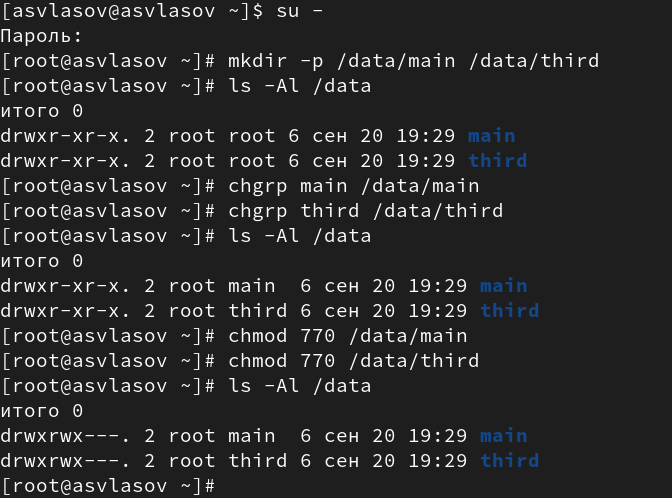
\includegraphics[width=0.7\textwidth,height=\textheight]{image/1.png}

}

\caption{Создание каталогов и прав доступа}

\end{figure}%

Заходим под учетной записью bob и создаем в каталоге main новый файл,
видим, что права доступа к этому файлу есть только у пользователя bob
так как он состоит в группе main.

\begin{figure}

{\centering 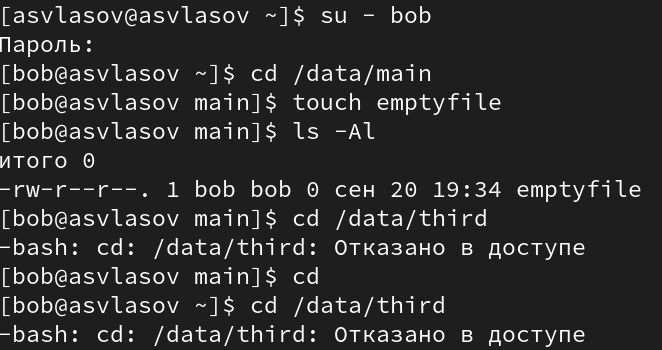
\includegraphics[width=0.7\textwidth,height=\textheight]{image/2.png}

}

\caption{bob}

\end{figure}%

В каталоге third мы не можем создать файл, так как bob не состоит в
группе third.

Создаем два новых файла через пользователя alice в каталоге main.

\begin{figure}

{\centering 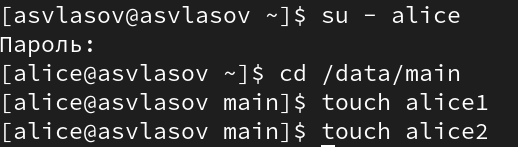
\includegraphics[width=0.7\textwidth,height=\textheight]{image/3.png}

}

\caption{alice new files}

\end{figure}%

Возвращаемся к пользователю bob и пытаемся удалить файлы пользователя
alice. Успешно, так как bob имеет полный доступ ко всем файлам
директории main.

\begin{figure}

{\centering 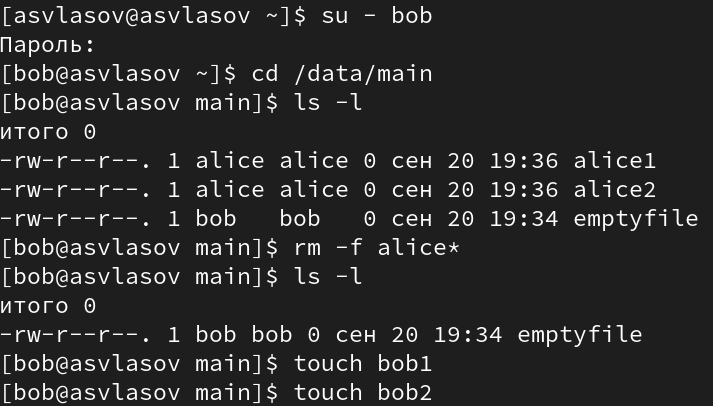
\includegraphics[width=0.7\textwidth,height=\textheight]{image/4.png}

}

\caption{Удаление файлов через bob}

\end{figure}%

Создаем два новых файла уже от пользователя bob.

Задаем новые права доступа для директории из учетной записи root.

\begin{figure}

{\centering 
\includegraphics[width=0.7\textwidth,height=\textheight]{image/5.png}

}

\caption{Новые права}

\end{figure}%

Пробуем создать новые файлы через пользователя alice - успешно. Пробуем
удалить файлы созданные учетной записью bob - отказано в доступе.

\begin{figure}

{\centering 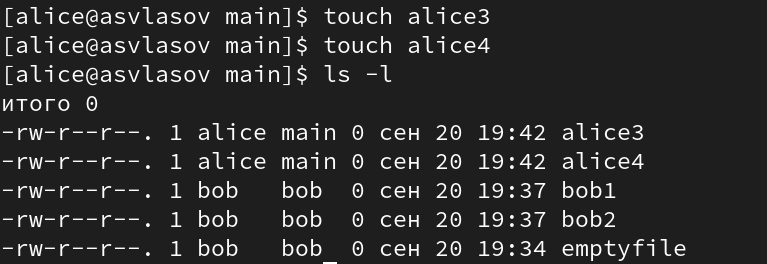
\includegraphics[width=0.7\textwidth,height=\textheight]{image/6.png}

}

\caption{Создание}

\end{figure}%

Теперь файлы пользователя bob принадлежат только ему и УЗ root, их
удаление другими пользователями невозможно.

\begin{figure}

{\centering 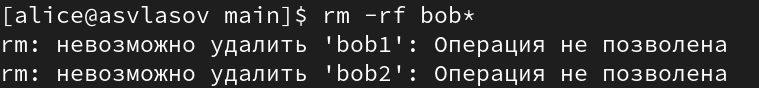
\includegraphics[width=0.7\textwidth,height=\textheight]{image/7.png}

}

\caption{Удаление}

\end{figure}%

Начинаем работу с ACL и задаем новые права доступа нашим директориям.

\begin{figure}

{\centering 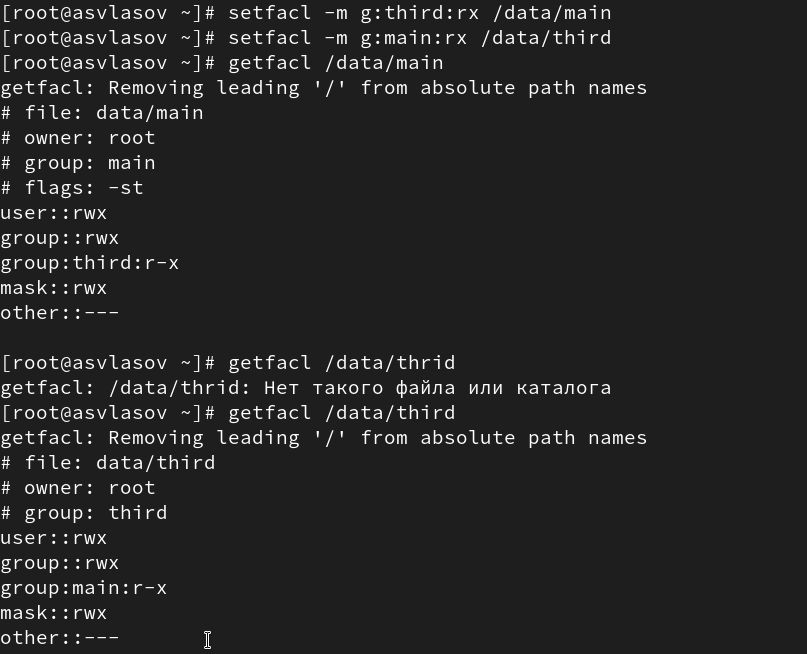
\includegraphics[width=0.7\textwidth,height=\textheight]{image/8.png}

}

\caption{ACL}

\end{figure}%

Теперь пользователям группы Third нельзя редактировать файлы каталога
main и наоборот.

Создаем новые файлы в наших директориях, видим что они доступны только
для чтения.

\begin{figure}

{\centering 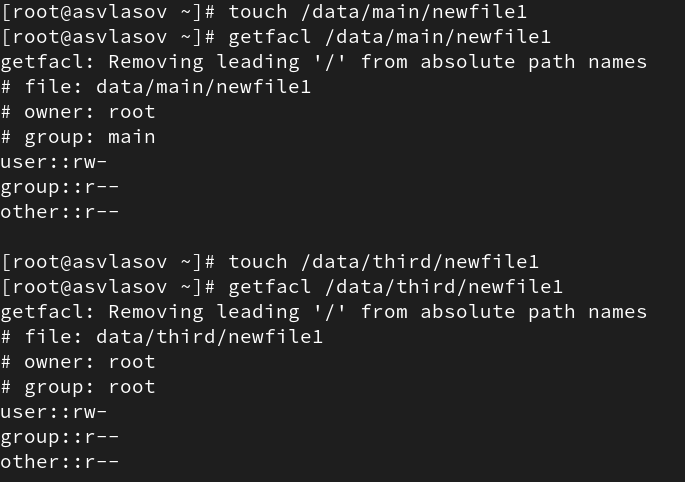
\includegraphics[width=0.7\textwidth,height=\textheight]{image/9.png}

}

\caption{Новые файлы}

\end{figure}%

Возвращаем значения ACL по умолчанию и проверяем права доступа. Создаем
два новых файла и видим отличия от первых двух. Теперь они доступны
полностью толкьто для пользователей соответствующей группы.

\begin{figure}

{\centering 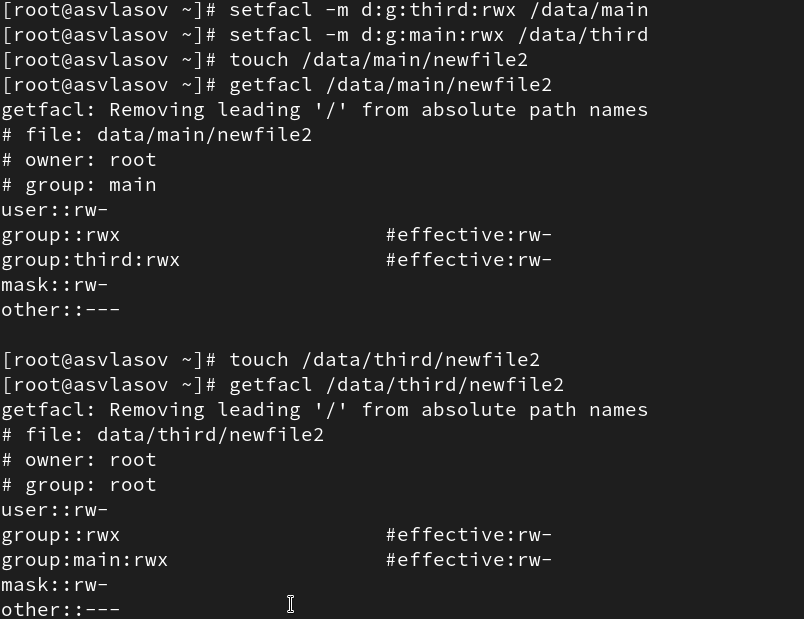
\includegraphics[width=0.7\textwidth,height=\textheight]{image/10.png}

}

\caption{Новые файлы и значения ACL}

\end{figure}%

Через пользователя carol пробуем удалить новые файлы, первый удалить
можно, а второй нет, так как carol находится в группе third.

\begin{figure}

{\centering 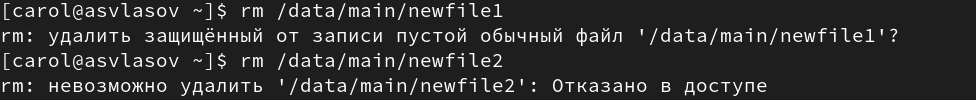
\includegraphics[width=0.7\textwidth,height=\textheight]{image/11.png}

}

\caption{Проверка заданных прав доступа}

\end{figure}%

Теперь пробуем записать текст в новые файлы через carol. Отказано в
доступе, так как у файла стоит щзапрет на редактирование для группы
third, редактирование второго успешно.

\begin{figure}

{\centering 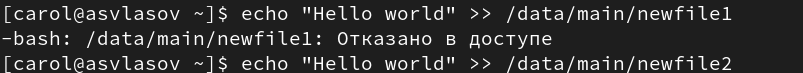
\includegraphics[width=0.7\textwidth,height=\textheight]{image/12.png}

}

\caption{Редактирование файлов}

\end{figure}%%
\begin{figure}

{\centering 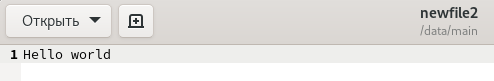
\includegraphics[width=0.7\textwidth,height=\textheight]{image/13.png}

}

\caption{Проверка редактирования}

\end{figure}%

\#Контрольные вопросы

\begin{enumerate}
\def\labelenumi{\arabic{enumi}.}
\item
  Как следует использовать команду chown, чтобы установить владельца
  группы для файла? chown :группа файл
\item
  С помощью какой команды можно найти все файлы, принадлежащие
  конкретному пользователю? find / -user имя\_пользователя
\item
  Как применить разрешения на чтение, запись и выполнение для всех
  файлов в каталоге /data для пользователей и владельцев групп? chmod -R
  ug=rwX /data (для каталогов) или chmod -R ug+rwx /data (точно для
  всех)
\item
  Какая команда позволяет добавить разрешение на выполнение для файла?
  chmod +x файл
\item
  Какая команда гарантирует наследование групповых разрешений для новых
  файлов? chmod g+s каталог
\item
  Как разрешить пользователям удалять только свои файлы в каталоге?
  chmod +t каталог (установка sticky bit)
\item
  Какая команда добавляет ACL на чтение для группы? setfacl -m
  g:группа:r *
\item
  Как гарантировать права на чтение для группы для всех текущих и
  будущих файлов? setfacl -R -m g:группа:rX . и setfacl -R -d -m
  g:группа:rX .
\item
  Какое значение umash нужно установить, чтобы «другие» не получали
  права? umask 007
\item
  Какая команда гарантирует, что никто не сможет удалить файл myfile?
  chattr +i myfile
\end{enumerate}

\chapter{Выводы}\label{ux432ux44bux432ux43eux434ux44b}

Мы получили навыки настройки базовых и специальных прав доступадля групп
пользователей в операционной системетипа Linux.

\chapter*{Список
литературы}\label{ux441ux43fux438ux441ux43eux43a-ux43bux438ux442ux435ux440ux430ux442ux443ux440ux44b}
\addcontentsline{toc}{chapter}{Список литературы}

\printbibliography[heading=none]




\end{document}
